\chapter{Evaluation und Einschränkungen}
\label{ch:Evaluation}
In diesem Kapitel wird das Evaluationsdesign und die Ergebnisse vorgestellt. Außerdem werden die Grenzen der Testbench aufgezeigt. Die Präsentation einer Zusammenfassung und potentiell zukünftiger Verbesserungen und Erweiterungen schließen diese Dokumentation ab.



\section{Evaluationsaufbau}
\label{sec:Evaluation:Aufbau}
Um die Testbench zu evaluieren, sind Experimente mit einem Auto-Skalierer auf realer Infrastruktur durchgeführt worden. Diese bestand dabei aus folgenden Komponenten: \\
Ein \textit{Workload-Service} in Form einer VM produziert eine reale Last, die über den \textit{Message-Broker} \textit{RabbitMQ}\footnote{https://www.rabbitmq.com/} an die Cloud-Service-Infrastruktur weitergegeben wird. Im speziellen wird hier die PaaS-Cloud von Bosch (\textit{Bosch IoT Cloud}) verwendet. In der Cloud befindet sich ein \textit{Python-Consumer} als skalierbarer Microservice, der diese Anfragen bearbeitet. Der verwendete Auto-Skalierer bekommt seine Metriken dabei von der Cloud-Infrastruktur, um so Instanzen des Microservices je nach Auslastung weg- oder hinzuzunehmen. Zwar ist die Implementierung des realen Auto-Skalierers eine Andere, von der Logik verhält er sich dennoch gleich.


%"l, b, r, t"
\begin{figure}[!h]
	\centering
	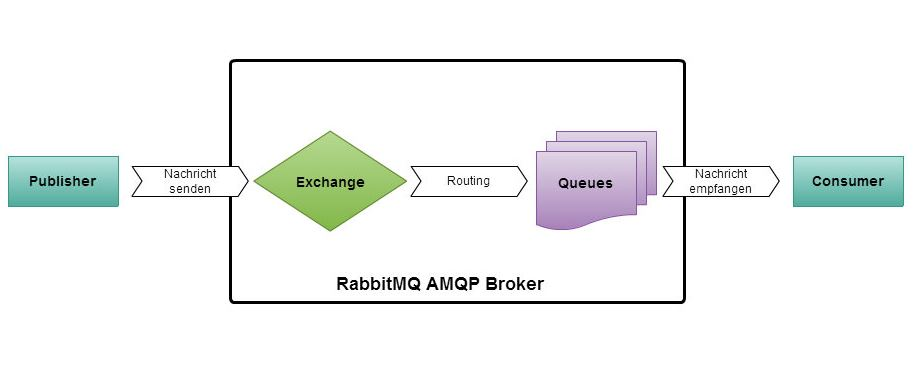
\includegraphics[width=13cm, trim={0cm 1.3cm 0cm 0.8cm}]{img/rabbitmq.jpg}
	\caption{RabbitMQ als Message-Broker, Quelle: \cite{rabbit}}
	\label{fig:rabbit}
\end{figure}

\noindent
Abbildung \ref{fig:rabbit} skizziert den Aufbau des \textit{Message-Brokers}. Der \textit{Publisher} ist dabei der \textit{Workload-Service} und der \textit{Consumer} der Microservice auf der \textit{Bosch IoT Cloud}, in dem der \textit{Python-Consumer} die Jobs verarbeitet. \\
Das CPU-Monitoring verhält sich wie folgt: Alle 10-15 Sekunden stehen pro Microservice-Instanz ein CPU-Update bereit. Daher ist die Auslastung zu Beginn nicht sofort auf 100\%, sondern erst nach 10 Sekunden auf 50\% und kurze Zeit später bei 100\% , auch wenn die Instanz bereits unter Volllast läuft. Erst nach ca. 20 Sekunden erhält man also die erste richtige Messung bei einer neuen Instanz. Dies ist deutlich anhand der gemessenen Werte (vgl. Abbildung \ref{fig:cpuResult}) erkennbar. Bei der Warteschlange wird ca. alle 5 Sekunden ein Update gemacht. \\
Basierend auf diesen Informationen wurden die Konfigurationsparameter erhoben. Nicht-spezifizierte oder nur implizit gegebene Parameter wurden geschätzt. Das genaue Anpassen aller Parameter ist jedoch nicht Teil des Praktikums, muss aber bei einer zielgenaueren Evaluation eines Auto-Skalierers gewissenhaft erledigt werden.




\section{Evaluationsergebnisse}
Die Abbildungen \ref{fig:vmsResult}, \ref{fig:cpuResult}, \ref{fig:queueLength} und \ref{fig:queueArrival} vergleichen die simulierten Werte (linke Spalte) mit der real gemessenen (rechte Spalte). Die Werte der jeweiligen Diagramme werden alle über die Zeit (x-Achse) aufgetragen. Die Einheit bei den Simulationsergebnissen ist über die Intervallnummer gegeben, die bei der realen Messung in Sekunden. 
Das Diagramm in Abbildung \ref{fig:vmsResult} beschreibt die Anzahl virtueller Maschinen über die Zeit. Es ist deutlich zu sehen, dass der Autoskalierer mit den simulierten Metriken, nahezu die selben Skalier-Entscheidungen trifft. \\
In Abbildung \ref{fig:cpuResult} wird die CPU-Auslastung aufgetragen. Auch hier stimmen die Simulationsergebnisse ziemlich genau mit der Realität überein. Wie in Sektion \ref{sec:Evaluation:Aufbau} beschrieben, weichen die ersten 20 Sekunden der real gemessenen Werte von der tatsächlichen Auslastung ab. Deshalb sind die simulierten Ergebnisse an dieser Stelle überraschenderweise sogar deutlich genauer. \\




%"l, b, r, t"
\begin{figure}[!h]
	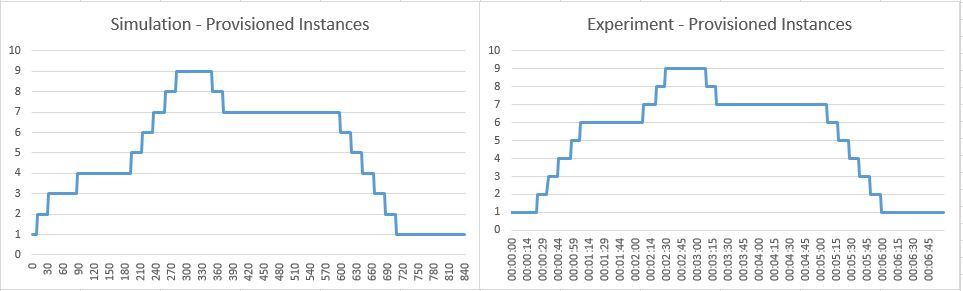
\includegraphics[width=\textwidth, trim={0cm 0cm 0cm 0cm}]{img/vms.jpg}
	\caption{Vergleich der Menge an Virtuellen Maschinen}
	\label{fig:vmsResult}
\end{figure}

%"l, b, r, t"
\begin{figure}[!h]
	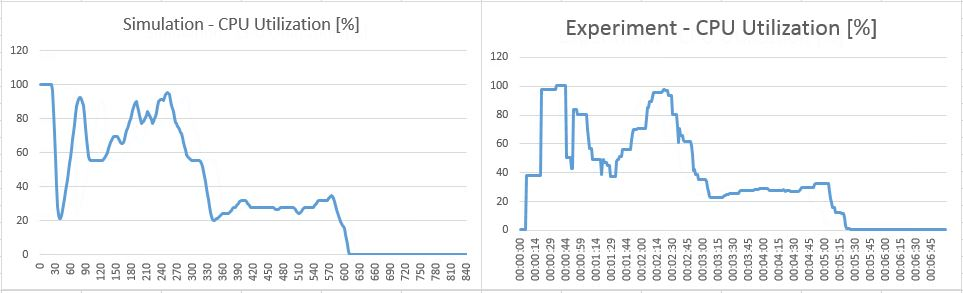
\includegraphics[width=\textwidth, trim={0cm 0cm 0cm 0cm}]{img/cpu.jpg}
	\caption{Vergleich der CPU Auslastung}
	\label{fig:cpuResult}
\end{figure}

\noindent
Das Diagramm in Abbildung \ref{fig:queueLength} vergleicht die simulierte und die tatsächliche Warteschlangen-Länge. Hier weichen die Simulationsergebnisse von der Realität ab. Dies liegt vor allem an der CPU: Da bei der realen Infrastruktur langsamer gemessen wird, werden vom Auto-Skalierer verzögerte Ressourcen provisioniert, wodurch die Warteschlangenlänge in der Realität schneller ansteigt.
. Dennoch ist die auch in der Simulation an den Ausschlägen zu erkennen, wann die Kapazität der Infrastruktur nicht ausreichend für die anliegende Last ist.\\
Ankunfts-und Verarbeitungsrate (Abbildung \ref{fig:queueArrival}) der Simulation stimmen hingegen mit der Realität relativ genau überein. Die Ankunftsrate (blaue Linie) der Simulation ist bis auf wenige nicht vorhandenen  Ausschläge ähnlich. Die Glättung der Kurve in der Simulation ist ein Effekt der Mittelwertbildung. 



%"l, b, r, t"
\begin{figure}[!h]
	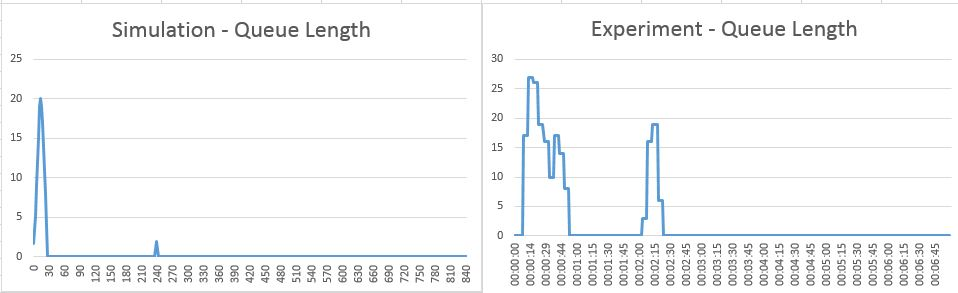
\includegraphics[width=\textwidth, trim={0cm 0cm 0cm 0cm}]{img/queueLength.jpg}
	\caption{Evaluationsergebnisse der Warteschlangenlänge}
	\label{fig:queueLength}
\end{figure}

%"l, b, r, t"
\begin{figure}[!h]
	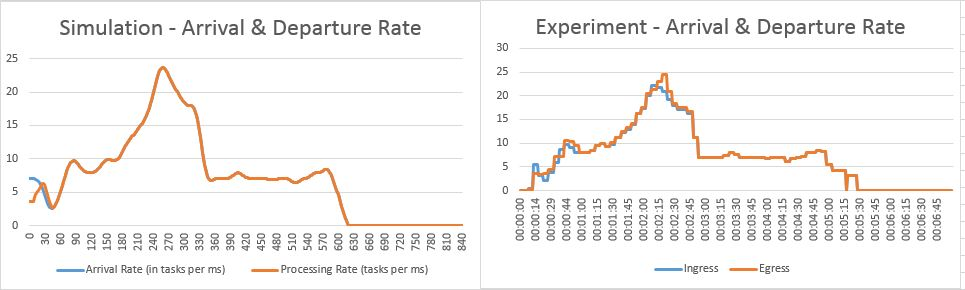
\includegraphics[width=\textwidth, trim={0cm 0cm 0cm 0cm}]{img/queueArrival.jpg}
	\caption{Evaluationsergebnisse der Ankunfts- und Verarbeitungszeit der Warteschlange}
	\label{fig:queueArrival}
\end{figure}



\section{Limitierungen}
Wie die Simulationsergebnisse zeigen, stimmen die Werte nicht zu 100\% mit der Realität überein. Dies ist der Tatsache geschuldet, dass die Parameter der Testbench nie genau bestimmt werden können. Beispielsweise wird vorausgesetzt, dass eine Virtuelle Maschine immer eine feste Zeit brauch, um ein Paket abzuarbeiten. VMs selbst sind aber auch nur eine weitere Abstraktion einer darunterliegenden Hardware-oder Software-Schicht, weshalb diese Annahme im Allgemeinen nicht gilt, denn die Verarbeitung eines Tasks kann durch eine darunterliegende Schicht pausiert werden. \\
Ein weiterer Grund ist die Umrechnung der externen Einheit [ms] auf die interne Einheit [Intervall], die oftmals mit Rundungsfehler behaftet ist. Dies ist insbesondere dann der Fall, wenn die Konfigurationsparameter nicht als Vielfache der Auflösung angegeben werden. Zwar mindert die interne Skalierung Rundungsfehler, kann sie aber nicht gänzlich eliminieren. \\
Ein weiterer Nachteil der aktuellen Implementierung ist die Gleichbehandlung aller Jobs. Es wird die vereinfachte Annahme gemacht, dass eine VM jeden Job in gleicher Zeit verarbeiten kann, was allerdings nicht der Realität entspricht. \\
Im Allgemeinen können viele Parameter nicht eindeutig bestimmt werden, da diese entweder nicht genau bekannt sind, oder aber nicht konstant sind.



\section{Zusammenfassung und Ausblick}
Das Ziel dieses Praktikums war es, eine Testbench zur Evaluation von Autoskalierern zu Entwickeln. Dafür wurde eine zeit-diskrete Simulations-Engine implementiert, die eine Cloud-Infrastruktur abstrahiert. Die wichtigsten Komponenten der Engine sind i) das \textit{InfrastructureModel}, das die Virtuellen Maschinen verwaltet und somit die Abarbeitung der Jobs simuliert ii) das \textit{QueueModel}, das eine Warteschlange darstellt, die sowohl ein Verzögerungsglied, wie auch ein Pufferspeicher simuliert iii) die \textit{MetricSource} als Komponente, die Metriken für einen Auto-Skalierer bereitstellt iv) ein Tracking-Mechanismus, der zeit-diskret die Informationen aller Komponenten abspeichert. Ein Auto-Skalierer ist ebenfalls Teil des Projektes, ist aber streng genommen kein Teil der Testbench, sondern wird nur über Schnittstellen an diese angebunden. \\
Nach der Implementierung der Applikation wurde ein Experiment durchgeführt. Dazu wurde eine spezifizierte Workload auf einer realen Infrastruktur getestet. Diese Infrastruktur wurde durch einen Auto-Skalierer dynamisch adaptiert, es wurden also je nach Last Virtuelle Maschinen instanziiert oder heruntergefahren. Das Verhalten der realen Komponenten ist dabei aufgezeichnet worden. Anschließend sind die Parameter der Infrastruktur und des Auto-Skalierers bestmöglich approximiert worden. Diese wurden als Eingabe-Konfiguration in die Testbench gegeben. Ebenso wurde die verwendete Workload als Eingabe verwendet. Die zu simulierende Zeit betrug 7 Minuten. Die Simulationszeit wenige Sekunden. \\
Der Vergleich der realen und der simulierten Ergebnisse ist höchst zufriedenstellend. Angemerkt werden sollte noch, dass die Simulation selbst in nur wenigen Sekunden durchgeführt werden konnte. Projiziert man dies auf ein deutlich längeres Intervall eines realen Experiments, so ist der Nutzen dieser Simulation deutlich absehbar. Weiterhin mussten für die Simulation keine Ressourcen einer Cloud-Infrastruktur genutzt werden, sondern lediglich ein Desktop-Rechner, auf dem diese durchgeführt wurde. \\
Für die Zukunft wäre es denkbar, ein geeignetes Frontend zu implementieren, sodass die Durchführung der Simulation benutzerfreundlicher ist. Vor allem die händische Eingabe der Parameter, beziehungsweise das (noch) etwas umständliche Anbinden eines anderen Auto-Skalierers kann durch eine geeignete Benutzeroberfläche deutlich erleichtert werden.










